%\documentclass[twocolumn]{emulateapj}
%\documentclass[12pt,preprint]{aastex}

\documentclass[usenatbib]{mn2e}

\newcommand{\s}{$_{\rm s}$}
\newcommand{\kms}{km~s$^{-1}$}
\newcommand{\msun}{{\it M}$_{\odot}$}
\newcommand{\lsun}{{\it L}$_{\odot}$}
\newcommand{\mear}{{\it M}$_{\oplus}$}
\newcommand{\etal}{{\it et al.}}
\newcommand{\ie}{{\it i.e.}}
\newcommand{\eg}{{\it e.g.}}
\newcommand{\be}{\begin{equation}}
\newcommand{\ee}{\end{equation}}
\newcommand{\magarc}{{\rm mag\,arcsec$^{-2}$}}
\newcommand{\MK}{{{\rm M}_{\rm ext,K}-5\log h}}
\newcommand{\ri}{{$r_{21}$}}
\newcommand{\ra}{$R_A$}
\newcommand{\vobs}{{v_{\rm obs}}}
\newcommand{\kmsMpc}{km~s$^{-1}$ Mpc$^{-1}$}
\newcommand{\h}{$h_{70}$}
\newcommand{\vpec}{v_{\rm pec}}
\newcommand{\like}{{\mathcal L}}
\newcommand{\vs}{\vspace*{5pt}}
\newcommand{\continued}{ (Continued)}

% Journals
%\newcommand{\mnras}{MNRAS}
%\newcommand{\apj}{ApJ}
%\newcommand{\apjl}{ApJL}
%\newcommand{\aj}{AJ}
%\newcommand{\pasp}{PASP}
%\newcommand{\aaps}{A\&AS}
%\newcommand{\aap}{A\&A}
%\newcommand{\apjs}{ApJS}
%\newcommand{\araa}{ARA\&A}
\newcommand{\pbar}{p_{\rm bar}}
\newcommand{\fHI}{f_{\rm HI}}

\voffset-1.25cm

\usepackage{epsfig}
\begin{document}

\title[Galaxy Zoo Hubble Data]{Galaxy Zoo: Classifications for Galaxies in HST Legacy Imaging}
%Bars Regulating Star Formation though the Atomic Gas Content of Disc Galaxies}
%The Atomic Gas Content of Barred Galaxies from ALFALFA$^*$: Bar Feedback in Intermediate Mass Disc Galaxies }
\author[Lead Author \etal]{Lead Author and other Galaxy Zoo science team\\
%$^1$Institute for Cosmology and Gravitation, University of Portsmouth, Dennis Sciama Building, Burnaby Road, Portsmouth, PO1 3FX, UK \\
%$^2$South East Physics Network, www.sepnet.ac.uk\\
%$^3$Dept. of Astronomy, Cornell University, Space Sciences Building, Ithaca, NY 14850, USA\\
 %$^2$Institute for Sciences of the Cosmos (ICCUB), University of Barcelona, Marti i Franques 1, Barcelona, 08024 Spain\\
% $^{4}$Oxford Astrophysics, Department of Physics, University of Oxford, Denys Wilkinson Building, Keble Road, Oxford, OX1 3RH, UK\\
%$^{5}$Yale Center for Astronomy and Astrophysics, Yale University, P.O. Box 208121, New Haven, CT 06520, USA \\
%$^6$Steward Observatory, University of Arizona, 933 N. Cherry Ave, Tuscon, AZ 85721, USA\\
 %$^4$Astronomy Department, Adler Planetarium and Astronomy Museum, 1300 Lake Shore Drive, Chicago, IL 60605, USA\\
 % $^7$Centre for Astronomy \& Particle Theory, University of Nottingham, University Park, Nottingham, NG7 2RD, UK\\
 %$^6$School of Physics and Astronomy, University of Minnesota, Minneapolis, MN 55455, USA\\
 %$^7$Department of Physics \& Astronomy, 206 Gallalee Hall, 514 University Blvd., University of Alabama, Tuscaloosa, AL 35487-0234, USA\\
% $^8$Einstein Fellow\\ 
\\
 $^*$This publication has been made possible by the participation of more than 200,000 volunteers in the Galaxy Zoo project. \\ Their contributions are individually acknowledged at \texttt{http://www.galaxyzoo.org/volunteers}. \\
\\
{\tt E-mail: lead.author@university.edu}
 }

%\date{Accepted for publication in MNRAS, 7th October 2010.}
%\pagerange{1--10} \pubyear{2010}

\maketitle

\begin{abstract}

This will be the data release paper for GZ Hubble. We present the classifications, the methodology for data reduction and corrections for redshift dependent biases in the observed morphologies. 

\end{abstract}

%\keywords{galaxies: distances and redshifts --- galaxies: clusters --- galaxies: fundamental parameters --- distance scale --- cosmological parameters}

\section{Introduction}


\section{Sample and Data} 

\subsection{Summary of HST Legacy Survey Imaging}

\begin{itemize}
\item AEGIS has 1 orbit each (~2200 seconds) in F606W (V band) and F814W filter and has been dithered to 0.03 ''/pixel; the imaging covers ~710 arcmin$^2$.

\item GOODS targeted 2 fields, GOODS-N and GOODS-S, imaging in 4 filters -- F435W (B), F606W (V), F775W (i), and F850LP (z). The mean exposure times vary, from 1000 - 2100 seconds. The images have been dithered to a pixel scale of 0.03 ''/pixel and covers at total area of ~320 arcmin$^2$ (160 arcmin$^2$ per field). The filters that Griffith et al uses for the colored images were F606W and F775W for GOODS-N and F606W and F850LP for GOODS-S.

\item COSMOS has 1 orbit (2028 seconds) in the F814W (I band) filter and has been dithered to 0.05 ''/pixel; it covers the largest area, ~1.8 deg$^2$. 

\item GEMS has 1 orbit (2160 and 2286 seconds) in the F606W and F850LP filters, with a pixel scale of 0.03 ''/pixel; it covers ~800 arcmin$^2$
\end{itemize}

\begin{table*}
\caption{Summary of GZ Hubble Samples \label{ferengi}}
\begin{tabular}{lclccc}
\hline\hline
Survey &  $t_{\rm exp}$ & Filters & Resolution & Area & $N_{\rm galaxies}$ \\
 & seconds & & \arcsec/pix & sq arcmin \\
\hline
AEGIS & 2200 & F606W (V) and F814W (I) & 0.03 & 710 \\
COSMOS & 2028 & F814W (I) & 0.05 & 6480\\
GEMS & 2160/2286 & F606W (V) and F850LP (z) & 0.03 & 800 \\
GOODS & 1000-2100s & F435W (B), F606W (V), F775W (i), F850LP (z) & 0.03 & 320 \\
\hline\hline
\end{tabular}
\end{table*}

\subsection{User Weighting}

The votes of individual users who classified galaxies in Galaxy Zoo Hubble are combined to make a vote fraction for each question on the classification tree. Users votes are weighted slightly (in a method identical to that described in Willett et al. 2013) such that users who frequently disagree with all other users end up having very low weights. The majority of users have weights very close to 1.0 ({\bf STEVEN: Is this true for GZH - do you have a plot of the distribution of user weights or consistencies we can include here?}. 

\section{Correcting for Redshift Dependent Classification Bias}

Previous version of Galaxy Zoo morphology classifications (Lintott et al. 2011, Willett et al. 2013) were based on observations of galaxies in the Sloan Digital Sky Survey (SDSS) which are typically at $z<0.1$. In these cases it could be assumed that there was no real evolution of the morphologies of galaxies and therefore any observed changes in the distribution of galaxies with different consensus morphologies was assumed to be due to the effects of redshift on the image quality (\ie. the reduction in physical resolution, surface brightness dimming etc). So for both previous releases of GZ morphogloies, a correction was provided for redshift dependent bias based on matching the classification fractions at the highest redshfts with those at the lowest redshift. See Bamford et al. (2009) and Willett et al. (2013) for the details. 

In the GZH samples the redshift range is so large that we expect to find redshift evolution of the types and morphologies of galaxies which are seen. So the previous methods of correcting for redshift dependent bias will not work. In addition the effects of band shifting will change the images even more across these redshift ranges. Figure \ref{redshift} which illustrates one possible effect of losing features in spiral galaxies at high redshift). 

%-----------------------------------------------------------------------------------------------------------------------------------
\begin{figure}
\begin{center}
\includegraphics[width=60mm]{example_ferengi2.ps}
%\includegraphics[height=80mm,angle=-90]{TuningFork.ps}
\caption{Examples of an obvious spiral and obvious elliptical at $z=0$ which both look similar when redshifted to $z=0.8$. See below for the description of the method for redshirting.  \label{exampleFERENGI}}
\end{center}
\end{figure}
 %-----------------------------------------------------------------------------------------------------------------------------------

In order to test the effects of redshift we made images of the same galaxy at a variety of redshifts using input images from the SDSS (cite the SDSS) and the FERENGI code (cite Ferengi) to produce images from these typical of those observed in the HST surveys. 
 
\subsection{Selection of FERENGI Input Galaxies}

We select 288 different galaxies in SDSS imaging to run through the FERENGI code.

The selection spanned a variety of galaxy morphologies (as indicated by GZ2 classifications), with a range of surface brightnesses, and also spanned the redshift range of SDSS targets (in $N_z = 4$ bins) in order to be optimised for different target minimum redshifts in HST imaging. 

 The selection criteria for the different morphological categories is summarised in Table \ref{morphologies}. The surface brightness selection ($N_\mu = 3$) was (1) low: $\mu > 21.5 {\rm mag arsec}^2$;  (2) mid: $20.5 < \mu < 21.5 {\rm mag arsec}^2$; and (3) high: $\mu < 20.5 {\rm mag arsec}^2$. 
 
\begin{table*}
\caption{Summary of morphological categories selected for FERENGI sample \label{morphologies}}
\begin{tabular}{lllc}
\hline\hline
Morphology & Label &  Selection & $N_{\rm objects}$ \\
 & & & ($N_z \times N_\mu$) \\
\hline
Features & Yes & $p_{\rm features} > 0.8$, $p_{\rm odd} < 0.1$ & 12 \\ 
 & Int & $0.3 < p_{\rm smooth} < 0.6$, $p_{\rm odd} < 0.1$ & 12 \\ 
 & No &  $p_{\rm smooth} > 0.8$, $p_{\rm odd} < 0.1$ & 12 \\ 
Merger & No & $p_{\rm features} > 0.8$, $p_{\rm odd < 0.1}$, $p_{\rm merger} < 0.1$ & 12\\
& Int & $p_{\rm odd} > 0.5$, $0.1< p_{\rm merger} < 0.4$ & 12 \\ 
& Yes & $p_{\rm odd} > 0.5$, $p_{\rm merger} > 0.4$ & 12\\
Edge-on & Yes &  $p_{\rm edgeon} > 0.8$, $p_{\rm features} > 0.5$ & 12 \\
& Int & $0.4 < p_{\rm edgeon} < 0.8$ , $p_{\rm features} > 0.5$ & 12 \\
& No & $p_{\rm edgeon} < 0.2$, $p_{\rm features} > 0.5$ & 12 \\
Bar & No & $p_{\rm bar} < 0.1$, $p_{\rm features} > 0.5$, $p_{\rm edgeon} < 0.2$ & 24 \\
& Int & $0.2 < p_{\rm bar} < 0.4$, $p_{\rm features} > 0.5$, $p_{\rm edgeon} < 0.2$ & 24 \\
& Yes&  $p_{\rm bar} > 0.8$, $p_{\rm features} > 0.5$, $p_{\rm edgeon} < 0.2$ & 24 \\
Visible spiral & No & $p_{\rm spiral} < 0.2$, $p_{\rm features} > 0.5$, $p_{\rm edgeon} < 0.2$, $p_{\rm bar} < 0.1$ & 12 \\
& Int &  $0.2 < p_{\rm spiral} < 0.8$, $p_{\rm features} > 0.5$, $p_{\rm edgeon} < 0.2$, $p_{\rm bar} < 0.1$ & 12 \\
& Yes &  $p_{\rm spiral} > 0.8$, $p_{\rm features} > 0.5$, $p_{\rm edgeon} < 0.2$, $p_{\rm bar} < 0.1$ & 12 \\
Oblique Bulge Size & No & $p_{\rm nobulge>0.6}$, $p_{\rm features} > 0.5$, $p_{\rm edgeon} < 0.5$, $p_{\rm bar} < 0.2$ & 12 \\
& Int &  $p_{\rm justnoticeable}>0.6$, $p_{\rm features} > 0.5$, $p_{\rm edgeon} < 0.5$, $p_{\rm bar} < 0.2$ & 12 \\
& Yes & $p_{\rm obvious/dominent}>0.5$\footnote{Edmond does this means $p_{\rm obv}+p_{\rm dom}>0.5$ or $p_{\rm ob} OR p_{\rm dom} >0.5$? }, $p_{\rm features} > 0.5$, $p_{\rm edgeon} < 0.5$, $p_{\rm bar} < 0.2$ & 12 \\
Edge-on bulge shape 
& Round & $p_{\rm rounded}>0.5$, $p_{\rm features} > 0.5$, $p_{\rm edgeon} > 0.5$ & 12\\
& Boxy & $p_{\rm boxy}>0.4$, $p_{\rm features} > 0.5$, $p_{\rm edgeon} > 0.2$ & 12\\
& Non & $p_{\rm nobulge}>0.5$, $p_{\rm features} > 0.5$, $p_{\rm edgeon} > 0.5$ & 12\\
\hline\hline
\end{tabular}
\end{table*}

For each of the four ``target redshifts" ($z = 0.3, 0.5, 0.8$ and 1.0), the images were redshifted in $\Delta z = 0.1$ bins up to $z=1.0$. In addition different evolution models were assumed in FERENGI. This evolution is a crude mechanism that is suppose to mimic the brightness increase of galaxies with increasing redshift. The evolution mechanism allows us to make galaxies brighter as linear function of redshift, and that is it. It is an empirical addition to the magnitude of a galaxy of the form $M' = e z + M$, where $M'$ is the corrected magnitude, $e$ is the evolutionary correction in magnitudes.  (i.e. $e=-1$ essentially brightens the galaxy by 1 magnitude by $z=1$). We ran FERENGI for values of $e$ starting from $e=0$ and decreasing to $e=-3.5$ in $\Delta e = 0.5$ steps. Depending on the target, or starting redshift we ran FERENGI for several final redshifts and different evolution models as summarized in Table \ref{ferengi}. 

\begin{table}
\caption{Summary of FERENGI runs \label{ferengi}}
\begin{tabular}{lcccccc}
\hline\hline
$z_{\rm target}$ &  $N_{z {\rm bins}}$ & $N_{\rm evolution}$ & $e_{\rm max}$ & $N_{\rm runs}$ & $N_{\rm total}$\\
\hline
0.3 & 8 & 7 & -3.0 & 56 & 4031 \\
0.5 & 6 & 4 & -1.5 & 24 & 1728 \\
0.8 & 3 & 3 & -1.0 & 9 & 648 \\
1.0 & 1 & 3 & -1.0 & 3 & 216 \\
\hline\hline
\end{tabular}
\end{table}

Two series of example redshifted images are shown in Figure \ref{exampleFERENGI}, both for runs with no evolution ($e=0$). 

\begin{figure*}
\includegraphics[width=160mm]{example_ferengi.ps}
%\includegraphics[height=80mm,angle=-90]{TuningFork.ps}
\caption{Examples of two galaxies which have been run through the FERENGI code to produce simulated HST images. The value of $p_{\rm features}$ for each panel is (1) Top row: $p_{\rm features}=$ 0.9, 0.625, 0.35, 0.35, 0.225 and (2) Bottom row: $p_{\rm features}=$ 1.00, 0.875, 0.875, 0.625, 0.375. \label{exampleFERENGI}}
\end{figure*}

 

\subsection{Results of FERENGI Analysis}

We show here the {\bf preliminary} results of citizen scientist classifications of images of galaxies placed at artificial redshifts. Figure \ref{results1} shows the {\bf preliminary} range of change of vote fractions for the change of $p_{\rm features}$ with redshift, for galaxies with different vote fraction levels, three ranges of surface-brightness levels and 7 evolutionary corrections (this last bit is indicated by the colour). 

%-----------------------------------------------------------------------------------------------------------------------------------
\begin{figure}
\begin{center}

\includegraphics[width=0.35\textwidth,angle=90]{somewhat_fake_results.ps}

\caption{Preliminary results of the FERENGI redshifting exercise. WARNING NO USER WEIGHTING.... For a range of vote fraction levels with three surface-brightness levels and 7 evolutionary corrections each (the colours indicate evolutionary correction value with green being $e=0$, we show the range of evolution of the vote fractions for featured vs. smooth with redshift.}

\label{fig:ferengi_results_fake}

\end{center}
\end{figure}
%-----------------------------------------------------------------------------------------------------------------------------------
\subsubsection{Results of Zeta Approach (Mel stuff)}

\begin{figure*}
\begin{center}
\includegraphics[width=\textwidth]{p_vs_p_SB_redshift.ps}
\caption{a caption. Add scale in $p_{\rm features}$ somehow that doesn't clutter the plot even more. }
\label{fig:p_vs_p}
\end{center}
\end{figure*}

In Figure \ref{fig:p_vs_p} we examine the change in $p_{\rm features}$ for the FERENGI images relative to their lowest simulated redshift ($\rm z_{sim}=0.3$). For each simulated redshift value $z$, and at fixed surface brightness $\mu$, we plot $p_{\rm features,z}$, the value measured at that simulated redshift, vs $p_{\rm features,z=0.3}$, the value measured for the same galaxy imaged at $z=0.3$. Only images corresponding to galaxies which also had FERENGI images at $z=0.3$ were included in this plot, which include 4031 out of the total 6624.
 
Our objective is to use these data to predict, for a galaxy with a measured $p_{\rm features,z}$ value, what its $p_{\rm features}$ value would have been if it had been viewed at $z=0.3$. This predicted value is defined as the debiased vote fraction $p_{\rm features,debiased}$, and is calculated by applying a correction to the measured value of $p_{\rm features}$, determined by the $\zeta$ function described in the previous section. We determine that a predicted value can be obtained so long as the relationship between $p_{\rm features,z}$ and $p_{\rm features,z=0.3}$ is single-valued; that is, for a given $p_{\rm features,z}$, there is one corresponding value of $p_{\rm features}$ at $z=0.3$. 

In Figure \ref{fig:p_vs_p} we see that the relationship between $p_{\rm features,z}$ and $p_{\rm features,z=0.3}$ is \emph{not} always single valued; hence we do not find it appropriate to correct galaxies that lie in these regions of surface brightness/redshift/$p_{\rm features}$ space. Our criteria for determining whether a region of this space is correctable is as follows: For each surface brightness and redshift bin, we examine the distribution of $p_{\rm features,z=0.3}$ for fixed $p_{\rm features,z}$ in bins of $\Delta p_{\rm features,z} = 0.1$. These sub-bins are marked by the horizontal lines within each larger, surface brightness/redshift bin. First, we require at least 5 points in each sub-bin to determine with confidence whether that region is correctable or uncorrectable. For the region to be considered correctable, we require that the inner two quartiles of the distribution of $p_{\rm features,z=0.3}$ within these sub-bins span a range less than 0.2. These regions are coloured purple, and the inner two quartile ranges are indicated by the black error bars within each sub-bin.If the spread is greater than 0.2, the region is considered uncorrectable; these are marked in green. Any region with fewer than 5 points is considered to have ``not enough information (NEI)'', and left uncoloured on the plot. 

Stuff to do in this section: 

\begin{itemize}
\item talk about where purple and green tend to be on plot, and about how green areas are primarily ellipticals and disks with all the features washed out - can't tell them apart! hence, can't debias
\item talk about where the Hubble sample falls in this space, reference table \ref{hubble_debiasable} 
\item justify N>5 and spread < 0.2 (or find a better way to choose criteria)
\item check out corrections for correctable and NEI, show some sample images of corrected galaxies
\item show some data for $p_{bar}$, determine or justify why we won't debiase them  
\end{itemize}
 
\begin{table}
\caption{Debiasable Hubble Stuff. Doesn't include SDSS yet. Note: stuff without good redshift info automatically gets put in uncorrectable category - which is about 25,000 galaxies. Might increase correctable number if we can get these measurements. \label{hubble_debiasable}}
\begin{tabular}{lrr}
\hline\hline
Category &  N & \% \\
\hline
Correctable   & 7408 & 6 \%  \\
Uncorrectable & 58526 & 50 \%\\
NEI           & 52149 & 44 \% \\
Total         & 118083 & 100 \% \\
\hline\hline
\end{tabular}
\end{table}


\subsubsection{TODO LIST}
We need to do: 
\begin{itemize}
\item Calculate the magnitudes, surface brightnesses and sizes of the galaxies in the FERENGI images....
\item Plot of magnitude distribution of galaxies in each of the four GZH subsamples with the magnitudes of our fake galaxies over plotted. 
\item Instructions of how to link the $z=0$ $p_X$ values for galaxies with a given size, magnitude (surface brightness) in the GZH images. 
\end{itemize}



\section{Summary}

Now people go and do science with these awesome Galaxy Zoo Hubble classifications.  
 
 
\paragraph*{ACKNOWLEDGEMENTS.} 

This publication has been made possible by the participation of more than 200,000 volunteers in the Galaxy Zoo project. Their contributions are individually acknowledged at \texttt{http://www.galaxyzoo.org/volunteers}. Galaxy Zoo 2 was developed with the help of a grant from The Leverhulme Trust. KS gratefully acknowledges support from Swiss National Science Foundation Grant PP00P2\_138979/1.

We thank ASIAA for hosting the ``Citizen Science in Astronomy" workshop, Mar 3-7th 2014 in Taipei, Taiwan, at which some of this analysis was done. 

HST acknowledgements.

Funding for the SDSS and SDSS-II has been provided by the Alfred P. Sloan Foundation, the Participating Institutions, the National Science Foundation, the U.S. Department of Energy, the National Aeronautics and Space Administration, the Japanese Monbukagakusho, the Max Planck Society, and the Higher Education Funding Council for England. The SDSS Web Site is http://www.sdss.org/. 

The SDSS is managed by the Astrophysical Research Consortium for the Participating Institutions. The Participating Institutions are the American Museum of Natural History, Astrophysical  Institute Potsdam, University of Basel, University of Cambridge, 
Case Western Reserve University, University of Chicago, Drexel University, Fermilab, the Institute for Advanced Study, the Japan 
Participation Group, Johns Hopkins University, the Joint Institute for Nuclear Astrophysics, the Kavli Institute for Particle Astrophysics and Cosmology, the Korean Scientist Group, the Chinese Academy of Sciences (LAMOST), Los Alamos National Laboratory, the Max-Planck-Institute for Astronomy (MPIA), the Max-Planck-Institute for Astrophysics (MPA), New Mexico State Uni- 
versity, Ohio State University, University of Pittsburgh, University of Portsmouth, Princeton University, the United States Naval Observatory and the University of Washington. 


\begin{thebibliography}{}

\end{thebibliography}

\end{document}
